\documentclass[   
state        = Report,                       % (Report | Slide    | Thesis)
lang         = EN,                           % (DE     | EN) 
degree       = MSc,                          % (BSc    | MSc)
dept         = MECH,                         % (MECH   | SBT)
bib-active   = true,                         % (true   | false)
bib-style    = ieee,                         % (ieee)
column-type  = one,                          % (one    | two)
]{mcidoc}

% CUSTOM COMMANDS -----------------------------------------------------------------------------
%       
% Please enter any custom command/packages you require here for easy tracking 
\usepackage[utf8]{inputenc}
\usepackage[T1]{fontenc}
\usepackage{mismath}
\usepackage{listings}
\usepackage{xcolor}
\usepackage{tabularx}
\usepackage{multirow}
\usepackage{makecell}
\usepackage{subcaption}
\usepackage{ifthen}
\usepackage{siunitx}
\usepackage{float}
\usepackage{hyperref}
\usepackage{tikz}
\usetikzlibrary{arrows.meta,calc,positioning}
\usepackage{pgfplots}
\pgfplotsset{compat=1.18}
\usepackage[european]{circuitikz} % 'european' für die Darstellung der Widerstände
% For example, bibliography setting are added. Bibtex is the standard but if you prefer
% there are other options on the market such as biber. Style has been chosen as IEEE but if 
% are from another discipline, please feel free to change it.

\bibliography{references.bib}  % Here we add our file where we store our references.
%      
% ---------------------------------------------------------------------------------------------

% DOCUMENT PARAMETERS -------------------------------------------------------------------------

\TitleHeader{Project Report}%   

\Title{%
  Adaptive Control of a DC-Motor 
}% 

\Lecture{Advanced Control Engineering II}%    

\Lecturer{Andreas Mehrle}%

\Cohort{MA-MECH-25}%           
\Group{MA-MECH-25-VZ}%

\StudentName{Felix Raffl,Lenard Wild}%



\begin{document} % ############################################################################\MakeTitlePage     

% REPORT CONTENT ------------------------------------------------------------------------------

% ----      
% Your report content should go here and should follow structure befitting of a scientific
% report and should be written in a scientific format. For more information please look at
% MCI guidelines on how it should be done.      
% ----  

% Include Chapter - introduction
\chapter{Adaptive Control of a Real DC Motor}
\section{Introduction}
In the previous example of the reader, the adaptive control of a DC-Motor is implemented on an Arduino Due using a first order model.
In this experiment the adaptive control of a DC-Motor is implemented on an ESP32 using a second order model. The hardware consists of an ESP32, an L298N H-bridge, and a DC motor with a quadrature encoder. For coding the ESP32, Simulink-Code-Generation is used. Figure \ref{fig:self-tuning-regulator-2nd-order} demonstrates the setup of the experiment. The plant parameters are estimated recursively, the controller is redesigned from these estimates, and the resulting incremental PI algorithm is executed on the ESP32 input/output interface.

\begin{figure}[htbp]
	\centering
	\resizebox{\linewidth}{!}{%
		\begin{tikzpicture}[
			auto,
			>=Latex,
			node distance=12mm and 14mm,
			block/.style={draw, rectangle, minimum height=9mm, minimum width=27mm, align=center},
			smallblock/.style={draw, rectangle, minimum height=8mm, minimum width=24mm, align=center},
			sum/.style={draw, circle, inner sep=0pt, minimum size=5.5mm},
			signal/.style={->, thick}
			]
			\node[sum] (sum) {};
			\node[left=10mm of sum] (r) {$r$};
			% Updated from PI to PID to handle second-order pole placement
			\node[block, right=13mm of sum] (pid) {incremental\\PID}; 
			\node[block, right=18mm of pid] (io) {ESP32\\I/O};
			\node[block, right=18mm of io] (plant) {DC motor\\and encoder};
			\node[right=22mm of plant] (y) {$y$};
			
			\node[smallblock, above=26mm of io] (pp) {pole\\placement};
			\node[smallblock, above=26mm of plant] (rls) {RLS\\estimator};
			
			\draw[signal] (r) -- (sum);
			\draw[signal] (sum) -- node {$e$} (pid);
			\draw[signal] (pid) -- node {$u$} (io);
			\draw[signal] (io) -- (plant);
			\draw[signal] (plant) -- (y);
			
			\coordinate (fbtap) at ($(plant.east)+(6mm,0)$);
			\coordinate (ytap)  at ($(plant.east)+(13mm,0)$);
			\coordinate (utap)  at ($(pid.east)+(5mm,0)$);
			\coordinate (uin)   at ($(rls.south)+(-6mm,0)$);
			\coordinate (yin)   at ($(rls.south)+(6mm,0)$);
			
			\draw[signal] (fbtap) |- ++(0,-13mm) -| node[pos=0.95, left] {$-$} (sum.south);
			
			\draw[signal] (utap) |- ($(uin)+(0,-11mm)$) -- (uin);
			\draw[signal] (ytap) |- ($(yin)+(0,-6mm)$) -- (yin);
			
			\fill (utap)  circle (0.6mm);
			\fill (ytap)  circle (0.6mm);
			\fill (fbtap) circle (0.6mm);
			
			% Updated to 4 parameters for a second-order ARX/ARMAX plant
			\draw[signal] (rls) -- node {$\hat a_1, \hat a_2, \hat b_1, \hat b_2$} (pp);
			
			\coordinate (dcorner) at ($(pp.south)+(0,-5mm)$);
			\coordinate (dturn)   at (pid.north |- dcorner);
			
			% Updated to 3 parameters for a PID controller
			\draw[signal] (pp.south) -- (dcorner)
			-- node[above] {$d_0, d_1, d_2$} (dturn) -- (pid.north);
		\end{tikzpicture}
	}
	\caption{Self-tuning regulator used for the ESP32 DC motor rig.}
	\label{fig:self-tuning-regulator-2nd-order}
\end{figure}
A more comprehensive DC motor model, accounting for electrical dynamics (armature inductance) in addition to mechanical dynamics, may be modeled as a second-order system. Normalizing the equation by dividing by $J L_a$ yields a standard monic form:
\begin{equation}
	\ddot{\omega} + \left(\frac{R_a}{L_a} + \frac{b}{J}\right)\dot{\omega} + \left(\frac{b R_a + K_m K_b}{J L_a}\right)\omega = \frac{K_m}{J L_a} u_{in}
\end{equation}

This translates into a general second-order continuous transfer function:
\begin{equation}
	G(s) = \frac{K}{(s + p_1)(s + p_2)}
\end{equation}

Discretization yields the discrete transfer function:
\begin{equation}
	G(z) = \frac{b_1 z + b_2}{z^2 + a_1 z + a_2}
\end{equation}

If we choose an incremental PID controller to handle the higher-order plant:
\begin{equation}
	G_C(z) = \frac{d_2 z^2 + d_1 z + d_0}{z(z - 1)}
\end{equation}

The closed-loop transfer function becomes:
\begin{equation}
	T(z) = \frac{(b_1 z + b_2)(d_2 z^2 + d_1 z + d_0)}{z^4 + (a_1 - 1 + b_1 d_2)z^3 + (a_2 - a_1 + b_1 d_1 + b_2 d_2)z^2 + (b_1 d_0 + b_2 d_1 - a_2)z + b_2 d_0}
\end{equation}

For a desired fourth-order denominator polynomial:
\begin{equation}
	q(z) = z^4 + q_3 z^3 + q_2 z^2 + q_1 z + q_0
\end{equation}

We equate the coefficients to derive the Diophantine system of equations. Solving top-down for the dominant controller parameters ($d_2, d_1, d_0$) yields:
\begin{equation}
	d_2 = \frac{q_3 - a_1 + 1}{b_1}
\end{equation}

\begin{equation}
	d_1 = \frac{q_2 - a_2 + a_1 - b_2 d_2}{b_1}
\end{equation}

\begin{equation}
	d_0 = \frac{q_1 + a_2 - b_2 d_1}{b_1}
\end{equation}
\section{The Test Rig}
The test rig, as can be seen in Figures \ref{fig:af2} and \ref{fig:af2}, is to be powered by a power supply with standard power jack connector, where the supply voltage must be greater than \SI{12}{\volt}, since the DC-Motor can be powered up to \SI{12}{\volt}. The voltage from the power supply is converted to \SI{12}{\volt} by a buck converter. The ESP32 is to be connected to the notebook via the USB type C connector, where the cable used can not be a USB-C to USB-C cable but rather a USB-A to USB-C, because of the pinout of the connector used in the ESP32 Dev Board.
\begin{figure}[H]
	\centering
	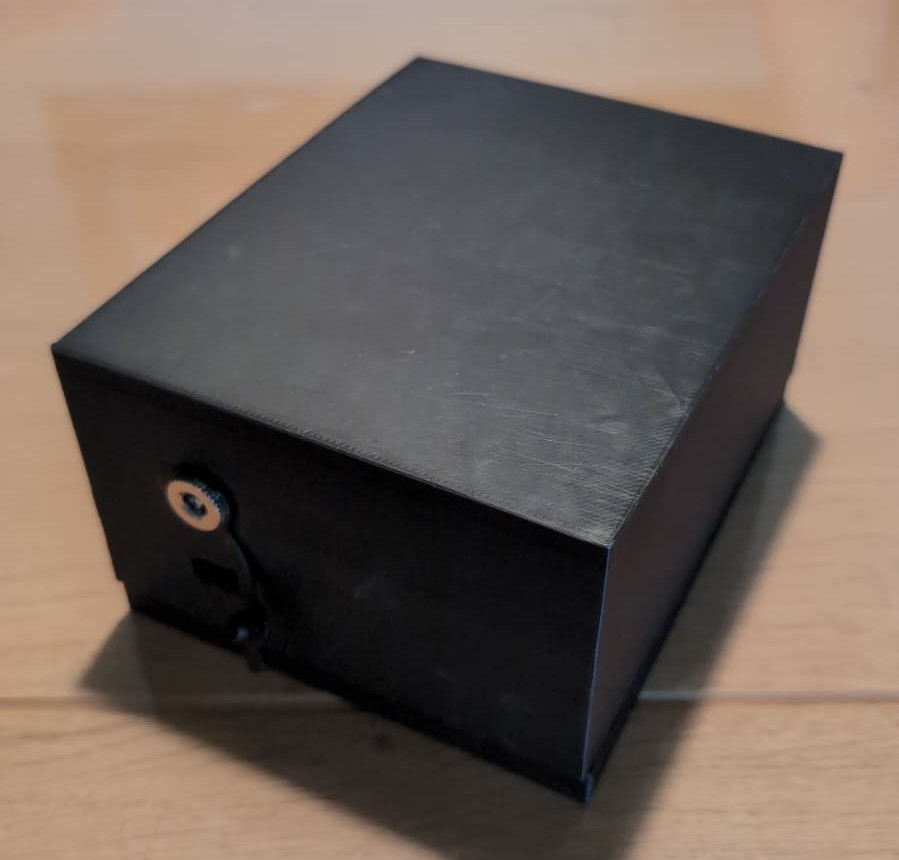
\includegraphics[width=0.7\textwidth]{figures/aufbau1.jpeg}
	\caption{}
	\label{fig:af1}
\end{figure}
\begin{figure}[H]
	\centering
	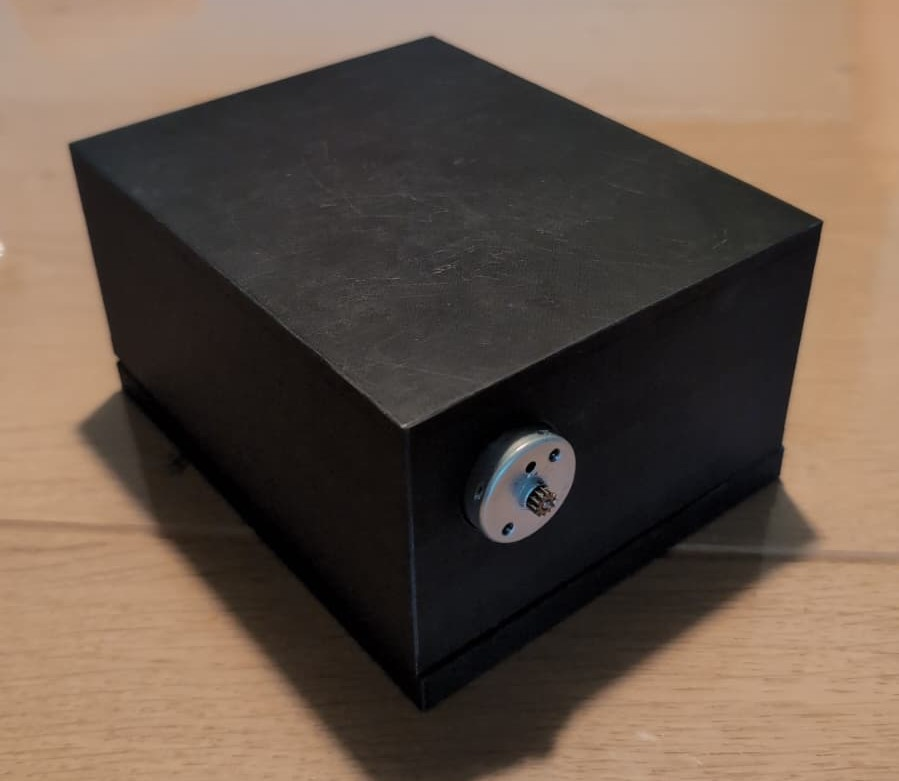
\includegraphics[width=0.7\textwidth]{figures/aufbau2.jpeg}
	\caption{}
	\label{fig:af2}
\end{figure}
\section{Measurements}

Figure \ref{fig:parameters} shows the convergence of the estimated plant parameters during operation.

\begin{figure}[H]
	\centering
	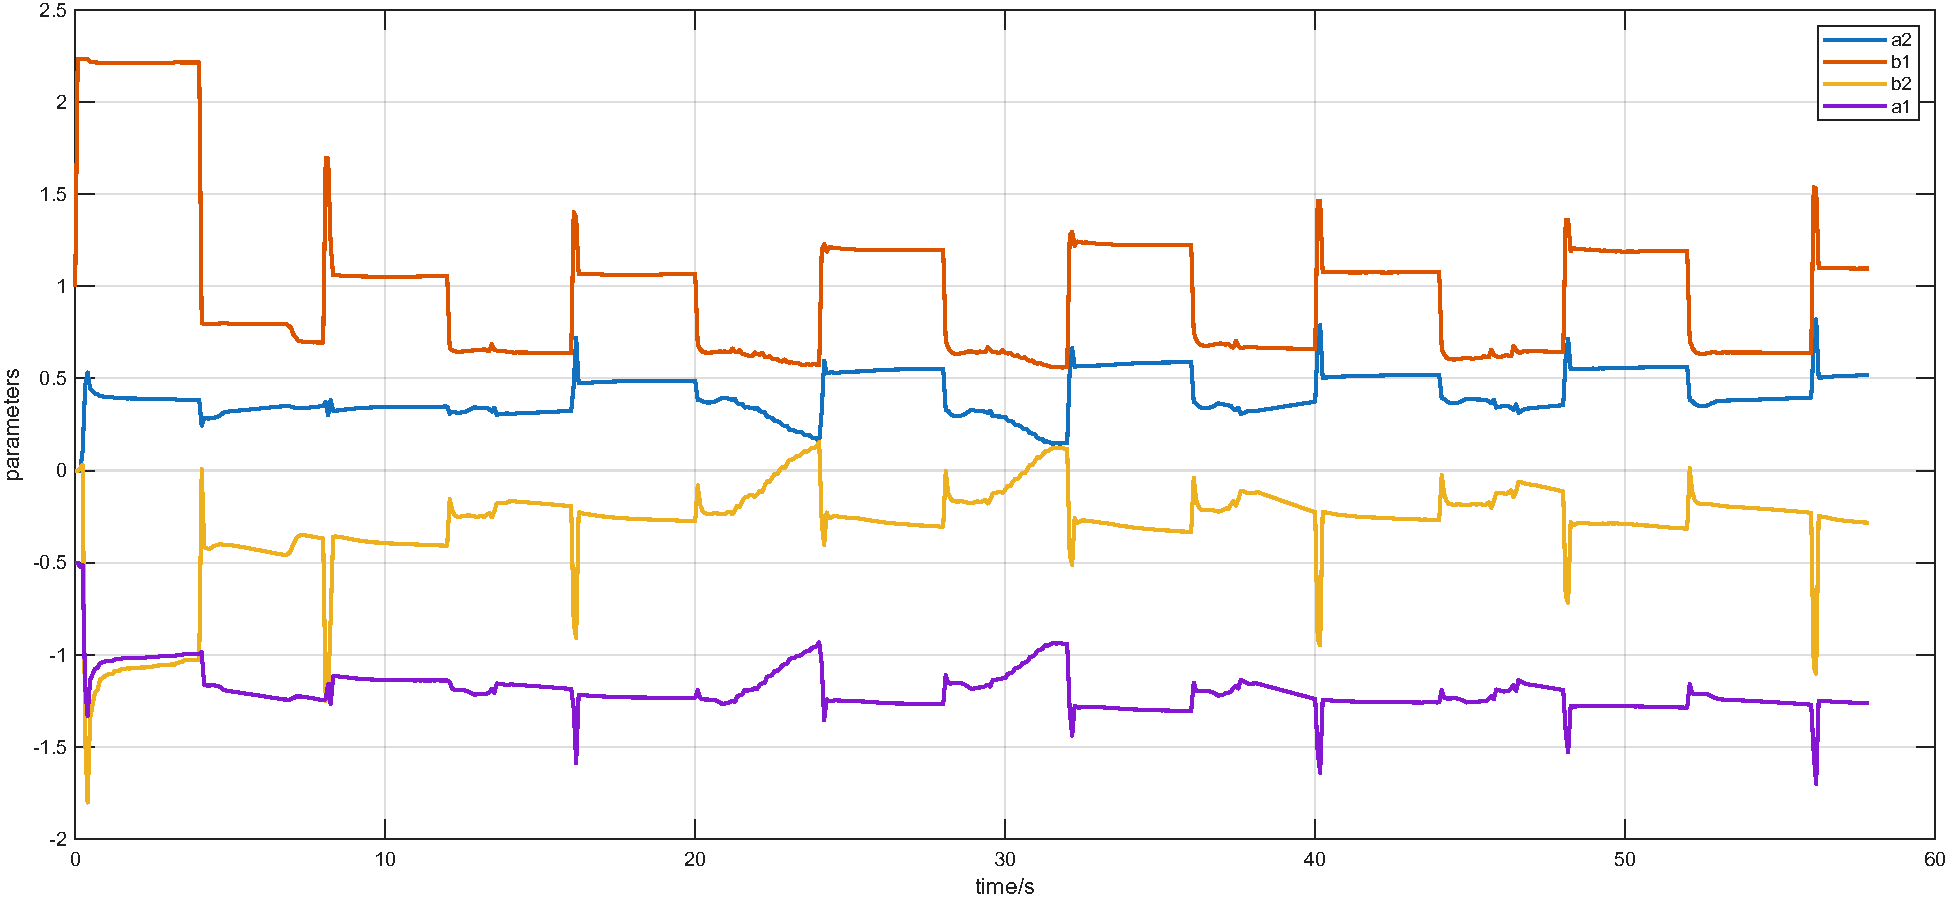
\includegraphics[width=\textwidth]{figures/parameters.pdf}
	\caption{Estimated parameters of the DC motor.}
	\label{fig:parameters}
\end{figure}

The corresponding closed-loop tracking response of the system is illustrated in Figure \ref{fig:response}.

\begin{figure}[H]
	\centering
	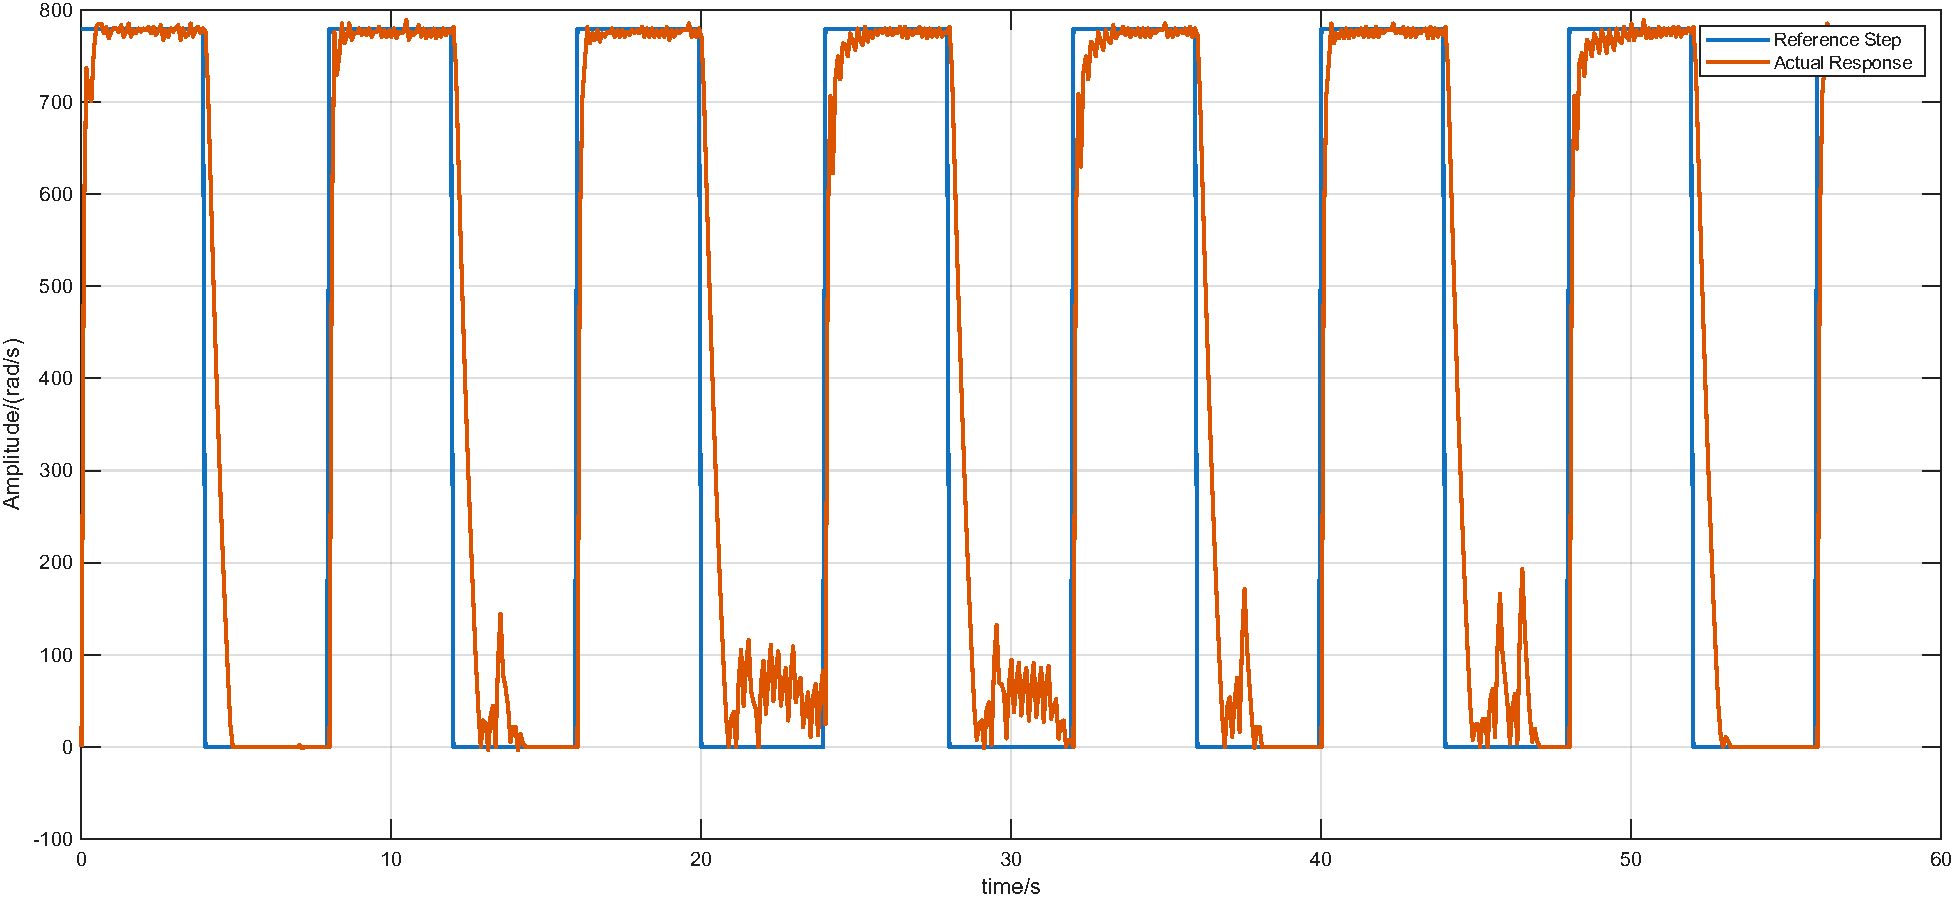
\includegraphics[width=\textwidth]{figures/response.pdf}
	\caption{Tracking response of the adaptive controller.}
	\label{fig:response}
\end{figure}   

% ---- 
% Add as many chapters as you see fit for your content. For easy legibility and for dynamic
% adjustment of content it would be suggested to write your files and place them similar to
% the aforementioned examples.

% REPORT POSTAMBLE ----------------------------------------------------------------------------


% ----


% \makeindex
% \printnomenclature
% \printglossaries

\end{document} % ##############################################################################
